\documentclass[border=15pt, multi, tikz]{standalone}
\usepackage{import}
\subimport{layers/}{init}
\usetikzlibrary{positioning}
\usetikzlibrary{3d} %for including external image 

\def\ConvColor{rgb:yellow,5;red,2.5;white,5}
\def\ConvReluColor{rgb:green,5;black,5}
\def\PoolColor{rgb:red,5;black,0.3}
\def\DcnvColor{rgb:blue,5;green,2.5;white,5}
\def\SoftmaxColor{rgb:magenta,5;black,7}
\def\FullyConnectedColor{rgb:magenta,5;black,7}
\def\SumColor{rgb:blue,5;green,15}

\begin{document}
\begin{tikzpicture}
\tikzstyle{connection}=[ultra thick,every node/.style={sloped,allow upside down},draw=\edgecolor,opacity=0.7]
%%%%%%%%%%%%%%%%%%%%%%%%%%%%%%%%%%%%%%%%%%%%%%%%%%%%%%%%%%%%%%%%%%%%%%%%%%%%%%%%%%%%%%%%
%% Draw Layer Blocks
%%%%%%%%%%%%%%%%%%%%%%%%%%%%%%%%%%%%%%%%%%%%%%%%%%%%%%%%%%%%%%%%%%%%%%%%%%%%%%%%%%%%%%%%Conversion failed! Please ensure that shell escape(standalone) is enabled (e.g. use '-shell-escape').

\node[canvas is zy plane at x=0] (temp) at (-5,0,0) {
	\centering
	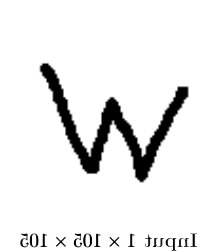
\includegraphics[width=8cm,height=8cm]{layers/input.png}
};

% conv1_1,conv1_2,%pool1
\pic[shift={(0,0,0)}] at (0,0,0) 
	{RightBandedBox={
		name=conv1,
		caption=\vspace{1.5cm} \\ conv \\ + \\ ReLU \\ + \\ MaxPool \\,
        xlabel={{"64",""}},
        ylabel=,
        zlabel=output $64 \times 48 \times 48$,
        fill=\ConvColor,
        bandfill=\ConvReluColor,%
        height=40,
        width=5,
        depth=40
	}
};
 
\pic[shift={(0,0,0)}] at (conv1-east) 
	{Box={
		name=pool1,%
        fill=\PoolColor,
        opacity=0.5,
        height=30,
        width=2,
        depth=30
    }
};
    
% conv2_1,conv2_2,pool2
\pic[shift={(3,0,0)}] at (pool1-east) 
	{RightBandedBox={
		name=conv2,
		caption=\vspace{4.3cm} \\ conv \\ + \\ ReLU \\ + \\ MaxPool \\,%
        xlabel={{"128",""}},
        zlabel=output $128 \times 21 \times 21$,
        fill=\ConvColor,
        bandfill=\ConvReluColor,%
        height=30,
        width=5,
        depth=30
    }
};
    
\pic[shift={(0,0,0)}] at (conv2-east) 
	{Box={
		name=pool2,%
        fill=\PoolColor,
        opacity=0.5,
        height=20,
        width=1,
        depth=20
    }
};
        
% conv3_1,conv3_2,pool3
\pic[shift={(3,0,0)}] at (pool2-east) 
	{RightBandedBox={
		name=conv3,
		caption=\vspace{7.0cm} \\ conv \\ + \\ ReLU \\ + \\ MaxPool \\,%
        xlabel={{"128","",""}},
        zlabel=output $128 \times 9 \times 9$,
        fill=\ConvColor,
        bandfill=\ConvReluColor,%
        height=20,
        width=5,
        depth=20
    }
};
    
\pic[shift={(0,0,0)}] at (conv3-east) 
	{Box={
		name=pool3,%
        fill=\PoolColor,
        opacity=0.5,
        height=10,
        width=1,
        depth=10
    }
};
    
% conv4_1,conv4_2,conv4_3,pool4
\pic[shift={(3,0,0)}] at (pool3-east) 
	{RightBandedBox={
		name=conv4,
		caption=\vspace{7.5cm} \\ conv \\ + \\ ReLU \\,%
        xlabel={{"256","",""}},
        zlabel=output $256 \times 6 \times 6$,
        fill=\ConvColor,
        bandfill=\ConvReluColor,%
        height=15,
        width=5,
        depth=15
    }
};

% fc1
\pic[shift={(3,0,0)}] at (conv4-east) 
	{Box={
	name=fc1,
	caption=\vspace{4.0cm}  \\ fc \\ + \\ sigmoid \\ + \\ $L_{1}$ siamese dist.,%
    xlabel={{"$1 \times 4096$", ""}},
    ylabel=,
    zlabel=,
    fill=\FullyConnectedColor,%
    height=35,
    width=2,
    depth=2
    }
};

         
%% fc2
\pic[shift={(3,0,0)}] at (fc1-east) {
	Box={
		name=fc2,
		caption=\vspace{9.0cm}  \\ fc \\ + \\ sigmoid,%
        xlabel={{"$1 \times 1$",""}},
        ylabel=,
        zlabel=,
        fill=\FullyConnectedColor,
        height=2,
        width=2,
        depth=2
	}
};  
        
%% Draw connections
%%%%%%%%%%%%%%%%%%%%%%%%%%%%%%%%%%%%%%%%%%%%%%%%%%%%%%%%%%%%%%%%%%%%%%%%%%%%%%%%%%%%%%%%
\draw [connection]  (pool1-east)    -- node {\midarrow} (conv2-west);
\draw [connection]  (pool2-east)    -- node {\midarrow} (conv3-west);
\draw [connection]  (pool3-east)    -- node {\midarrow} (conv4-west);
\draw [connection]  (conv4-east)    -- node {\midarrow} (fc1-west);
\draw [connection]  (fc1-east)    -- node {\midarrow} (fc2-west);

%%%%%%%%%%%%%%%%%%%%%%%%%%%%%%%%%%%%%%%%%%%%%%%%%%%%%%%%%%%%%%%%%%%%%%%%%%%%%%%%%%%%%%%

\end{tikzpicture}
\end{document}\grid
